\chapter{DSP Configuration (SigmaStudio)}
\label{ch:sigmastudio}

This chapter documents how the ADAU1701 is configured in SigmaStudio: the
hardware settings that must match the board, the audio signal-processing
chain, and the parameters exposed for runtime control by the ESP32. The
resulting SigmaStudio export is what the host writes into the DSP's RAM at
every boot (Section~\ref{sec:hw-adau}). For the firmware driver, safeload
API, persistence, and HTTP usage, see Chapter~\ref{ch:adau1701}.

\section{Overview}
\label{sec:ss-overview}

The DSP program is built once in SigmaStudio and exported as a sequence of
register writes. Because the board carries no self-boot EEPROM, the ESP32
replays that sequence over I\textsuperscript{2}C (address 0x34) on every
power-up. SigmaStudio is therefore used purely to \emph{design and export}
the program, not to drive the chip in operation.

\begin{drkey}[No hardware required to export]
The whole program can be built and exported offline, without a physical
ADAU1701 or a USBi programmer connected. A USBi block is placed in the
Hardware Configuration only because SigmaStudio requires a communication
channel to compile.
\end{drkey}

\begin{drref}[Live connection is also possible]
Since firmware~0.9.0, DigiRadio's \texttt{net::SigmaStudioTcpServer}
(Chapter~\ref{ch:adau1701}, Section~\ref{sec:adau1701-sigmastudio-tcp})
exposes a TCP:8086 bridge so SigmaStudio can \emph{Connect} and
\emph{Link Compile Download} directly against a running board, for live DSP
tuning and bench debugging. The export-only workflow below remains the
simplest path for ordinary firmware builds.
\end{drref}

\section{Hardware Configuration}
\label{sec:ss-hwcfg}

The Hardware Configuration tab must mirror the board exactly. The key
settings are collected in Table~\ref{tab:ss-hwcfg}. The 48\,kHz system
sample rate follows from the \textbf{board strapping}, not from a
SigmaStudio preference alone: X1 is a 12.288\,MHz crystal, PLL\_MODE selects
256\,$\times$\,f\textsubscript{S}, and 12.288\,MHz\,/\,256 = 48\,kHz.

\begin{table}[htbp]
  \centering
  \begin{tabular}{@{}L{4.2cm}L{9.2cm}@{}}
    \drhead Setting & Value \\
    \midrule
    Control port (I\textsuperscript{2}C address) & 0x34 (ADDR0/ADDR1 = GND) \\
    Self-boot                     & Disabled (host RAM load) \\
    System sample rate            & 48\,kHz (256\,$\times$\,f\textsubscript{S} strapping) \\
    MCLK                          & 12.288\,MHz crystal (256\,$\times$\,f\textsubscript{S}) \\
    Serial Input format           & I\textsuperscript{2}S, 24-bit \\
    Serial Output                 & \textbf{Master Mode} (ADAU generates clocks) \\
    Word length                   & 24 bits \\
    RAM Modulo / Program Length   & 1x (1024 instructions) \\
    \bottomrule
  \end{tabular}
  \caption{ADAU1701 hardware settings in SigmaStudio.}
  \label{tab:ss-hwcfg}
\end{table}

\begin{drnote}[Clock source on the board]
SigmaStudio's 48\,kHz sample-rate field must agree with the fabricated
hardware: passive crystal X1 (12.288\,MHz, CL = 12\,pF) on MCLKI/OSCO with
22\,pF load caps, PLL\_MODE0 = GND and PLL\_MODE1 = 3V3 (256\,$\times$\,f\textsubscript{S}).
The ADAU1701 internal oscillator multiplies the crystal; it is not an active
oscillator module. See Chapter~\ref{ch:hardware}, Section~\ref{sec:hw-val-adau}.
\end{drnote}

\subsection{Multipurpose pin (MP) assignment}

The ADAU1701 multipurpose pins are assigned to the serial audio signals
as wired on the board. Table~\ref{tab:ss-mp} lists the assignment; it
matches the board GPIO map (Section~\ref{sec:hw-gpio}).

\begin{table}[htbp]
  \centering
  \begin{tabular}{@{}L{2.4cm}L{3.6cm}L{7.2cm}@{}}
    \drhead MP pin & Direction / function & Signal \\
    \midrule
    MP0  & Input Sdata\_in0     & audio from Si4684 (radio) \\
    MP1  & Input Sdata\_in1     & audio from ESP32 \\
    MP4  & Input Lrclk\_in      & LRCLK (returned via board link) \\
    MP5  & Input Bclk\_in       & BCLK (returned via board link) \\
    MP6  & Output Sdata\_out0   & audio to FSC-BT1035 \\
    MP10 & Lrclk\_out           & LRCLK generated (master) \\
    MP11 & Bclk\_out            & BCLK generated (master) \\
    \bottomrule
  \end{tabular}
  \caption{Multipurpose pin assignment. MP2, MP3, MP7--MP9 are unused
    (GPIO input, default).}
  \label{tab:ss-mp}
\end{table}

\begin{drnote}[Master clock routing]
The ADAU1701 is the I\textsuperscript{2}S master: it generates LRCLK and
BCLK on MP10/MP11. On the board these are wired to MP4/MP5, so the same
master clocks time the serial inputs. This shared-clock scheme means the
serial inputs are configured as \emph{clock inputs} even though the ADAU
itself is master --- the clocks originate at MP10/MP11 and return through
the board link. All companion chips (Si4684, ESP32, BT1035) are
I\textsuperscript{2}S slaves.
\end{drnote}

\section{Signal-processing chain}
\label{sec:ss-chain}

The audio flows through a fully stereo chain, built in the Schematic tab
(Figure~\ref{fig:ss-chain}). Two stereo sources are level-trimmed, mixed,
equalised, volume-controlled, and peak-limited before reaching the two
digital outputs that feed the Bluetooth module.

\begin{figure}[htbp]
  \centering
  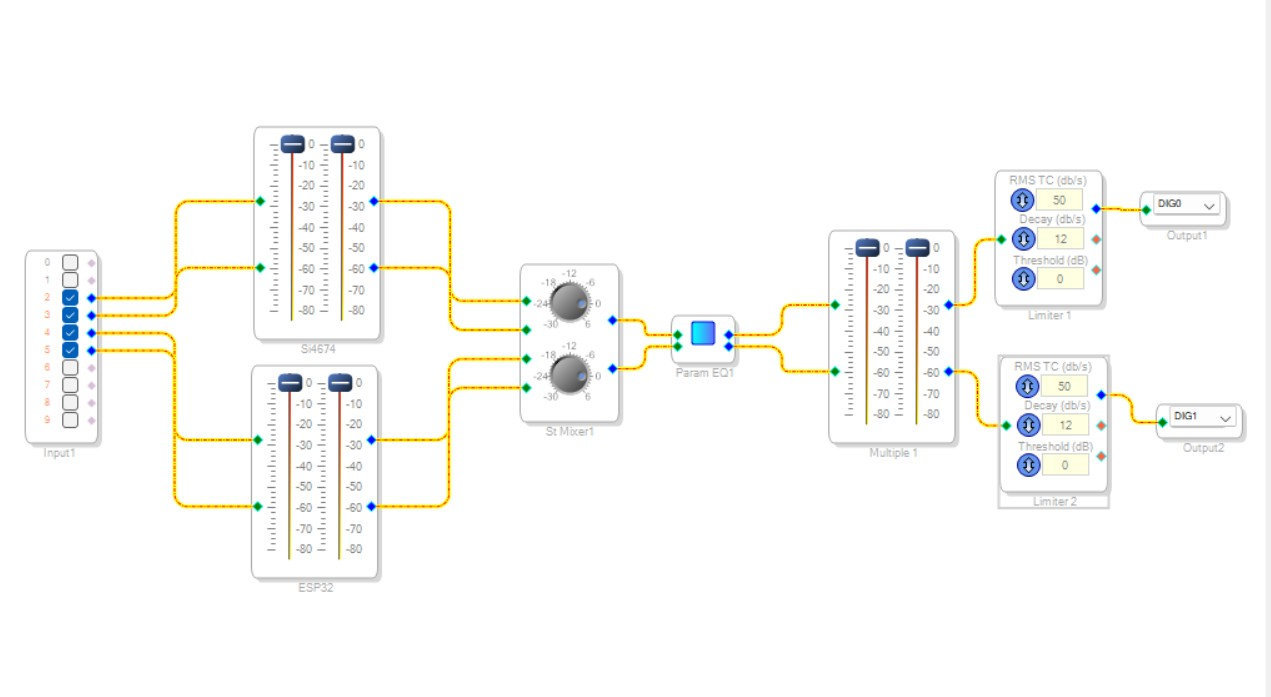
\includegraphics[width=\linewidth]{sigma-chain.jpg}
  \caption{The complete stereo signal-processing chain in SigmaStudio:
    Input \(\rightarrow\) source faders \(\rightarrow\) stereo mixer
    \(\rightarrow\) parametric EQ \(\rightarrow\) master volume
    \(\rightarrow\) per-channel limiters \(\rightarrow\) outputs.}
  \label{fig:ss-chain}
\end{figure}

\subsection{Block-by-block}

\begin{table}[htbp]
  \centering
  \small
  \begin{tabular}{@{}L{2.4cm}L{3.6cm}L{7.2cm}@{}}
    \drhead Stage & Block & Role \\
    \midrule
    Input      & Input (ch. 2--5)          & radio L/R, ESP32 L/R \\
    Source trim & Si4674, ESP32 faders     & per-source stereo level \\
    Mix        & Stereo Mixer             & combine sources, keep L/R \\
    EQ         & Parametric EQ (2-ch)     & high-pass + 5 peaking bands \\
    Volume     & Multiple volume (2-ch)   & master volume \\
    Protect    & Limiter 1 / Limiter 2    & per-channel peak limiting \\
    Output     & Output (DIG0, DIG1)      & L/R to FSC-BT1035 \\
    \bottomrule
  \end{tabular}
  \caption{Signal-processing blocks and their roles. The chain is stereo
    end to end; L and R never collapse to mono.}
  \label{tab:ss-blocks}
\end{table}

\subsection{Signal flow}

\begin{drcode}[Signal flow (stereo)]
Input ch2/3 (radio L/R)  -> Si4674 fader  --.
                                            |-> Stereo Mixer -> Param EQ
Input ch4/5 (ESP32 L/R)  -> ESP32  fader  --'
   -> Master Volume -> Limiter L / Limiter R -> Output DIG0 / DIG1 -> BT1035
\end{drcode}

\section{Equaliser}
\label{sec:ss-eq}

The parametric EQ is a two-channel (stereo) block; a single set of bands
applies identically to L and R. It is configured with one high-pass and
five peaking bands, all starting flat (0\,dB) so the default response is
neutral and any tone shaping is an explicit choice made at runtime by the
firmware.

\begin{table}[htbp]
  \centering
  \footnotesize
  \begin{tabular}{@{}L{1.4cm}L{2.4cm}L{2.2cm}L{1.6cm}L{1.2cm}@{}}
    \drhead Band & Type & Frequency & Gain & Q \\
    \midrule
    1 & HP Butterworth & 20\,Hz   & ---   & 1.41 \\
    2 & Peaking                      & 100\,Hz  & 0\,dB & 1.0 \\
    3 & Peaking                      & 400\,Hz  & 0\,dB & 1.0 \\
    4 & Peaking                      & 1\,kHz   & 0\,dB & 1.0 \\
    5 & Peaking                      & 3\,kHz   & 0\,dB & 1.0 \\
    6 & Peaking                      & 8\,kHz   & 0\,dB & 1.0 \\
    \bottomrule
  \end{tabular}
  \caption{Parametric EQ bands. Band~1 removes DC and subsonic content;
    bands 2--6 are the tone controls the firmware adjusts.}
  \label{tab:ss-eq}
\end{table}

\begin{drnote}[Double precision for the high-pass]
The high-pass sits at 20\,Hz, very low relative to the 48\,kHz sample
rate, so it uses a double-precision second-order block to avoid
coefficient-quantisation noise in the bass. The peaking bands can use
single precision.
\end{drnote}

\section{Master volume and limiters}
\label{sec:ss-vol}

A two-channel volume block provides the master level (0\,dB default). Two
single-channel limiters --- one per channel --- protect the FSC-BT1035
input from clipping on peaks. Suggested limiter settings are in
Table~\ref{tab:ss-lim}.

\begin{table}[htbp]
  \centering
  \begin{tabular}{@{}L{4.2cm}L{9.2cm}@{}}
    \drhead Parameter & Value \\
    \midrule
    RMS TC        & 50\,dB/s \\
    Decay         & 12\,dB/s \\
    Threshold     & $-1$\,dB (protective) \\
    \bottomrule
  \end{tabular}
  \caption{Per-channel limiter settings. The limiter is left fixed (not
    runtime-adjustable).}
  \label{tab:ss-lim}
\end{table}

\section{Runtime-controllable parameters}
\label{sec:ss-runtime}

The firmware controls a subset of the DSP at runtime via safeload writes.
These are the parameter cells whose addresses must be recorded from the
SigmaStudio export (Section~\ref{sec:ss-export}).

\begin{table}[htbp]
  \centering
  \begin{tabular}{@{}L{2.4cm}L{3.6cm}L{7.2cm}@{}}
    \drhead Control & Block & Runtime-adjustable \\
    \midrule
    Source levels (2)   & Si4674 / ESP32 faders & yes \\
    EQ bands 2--6       & Parametric EQ         & yes (gain/freq/Q) \\
    Master volume       & Multiple volume       & yes \\
    High-pass (band 1)  & Parametric EQ         & fixed \\
    Limiters            & Limiter 1 / 2         & fixed \\
    \bottomrule
  \end{tabular}
  \caption{Parameters exposed to the firmware. Fixed blocks are set once
    in the program and never written at runtime.}
  \label{tab:ss-runtime}
\end{table}

\section{Virtual enhancements (stereo depth and bass boost)}
\label{sec:ss-enhancements}

The SigmaStudio export does not include dedicated stereo widener or bass
boost blocks. Firmware maps enhancement levels (0--100) onto the
existing Param EQ1 bands at runtime:

\begin{itemize}
  \item \textbf{Bass enhance} --- peaking boost at 100\,Hz (+9\,dB max)
        and 400\,Hz (+3\,dB max).
  \item \textbf{Stereo enhance} --- slight 1\,kHz cut, plus 3\,kHz and
        8\,kHz lift for a wider, more present image. This is a
        psychoacoustic curve, not mid/side processing.
\end{itemize}

Enhancement levels are stored in \texttt{AudioProfile::enhancements} and
applied by \texttt{core::applyEnhancementsToEq()} before safeload. Base EQ
band settings in NVS are preserved; overlays replace affected bands only
while the corresponding level is greater than zero.

\begin{drcaution}[Use safeload for live changes]
All runtime updates to the volume, source levels, and EQ bands must go
through the ADAU1701 safeload mechanism. Writing parameter cells directly
while audio is playing produces audible clicks.
\end{drcaution}

\section{Exporting the program}
\label{sec:ss-export}

With the schematic complete, the program is exported for the firmware:

\begin{enumerate}
  \item Enable \emph{Action \(\rightarrow\) Enable Short Parameter Name
        for Export} so the exported cell names are concise.
  \item \emph{Action \(\rightarrow\) Export System Files}, and choose an
        output folder.
\end{enumerate}

The export produces the program data (control registers, program RAM, and
parameter RAM) as byte sequences, plus the symbolic parameter addresses.
The firmware's ADAU1701 driver replays the program data over
I\textsuperscript{2}C at boot, and uses the parameter addresses for
safeload updates.

\begin{drnote}[Export System Files vs. Link Compile Download]
Without a physical ADAU1701/USBi attached, \emph{Export System Files} is what
you want: it compiles the schematic and writes the files directly, with no
chip connection required. \emph{Link Compile Download} instead needs a live
communication channel to a chip --- either the classic USBi/ICP dongle, or
DigiRadio's own TCP:8086 SigmaStudio bridge (Section~\ref{sec:adau1701-sigmastudio-tcp})
when connecting live to a running board.
\end{drnote}

\section{Next revision: DigiRadioFinale}
\label{sec:ss-digiradiofinale}

\begin{drcaution}[Not yet integrated into firmware]
This section documents a SigmaStudio export (\texttt{DigiRadioFinale}) captured
2026-08-25 that is not yet the program the firmware replays at boot. It expands
the parameter RAM from 74 to 224 words with several new dedicated blocks,
replacing two of the EQ-overlay workarounds in
Section~\ref{sec:ss-enhancements} with real ADI algorithm modules. Driver,
safeload API, and this manual's runtime tables will be updated once the
program is finalised.
\end{drcaution}

\begin{figure}[htbp]
  \centering
  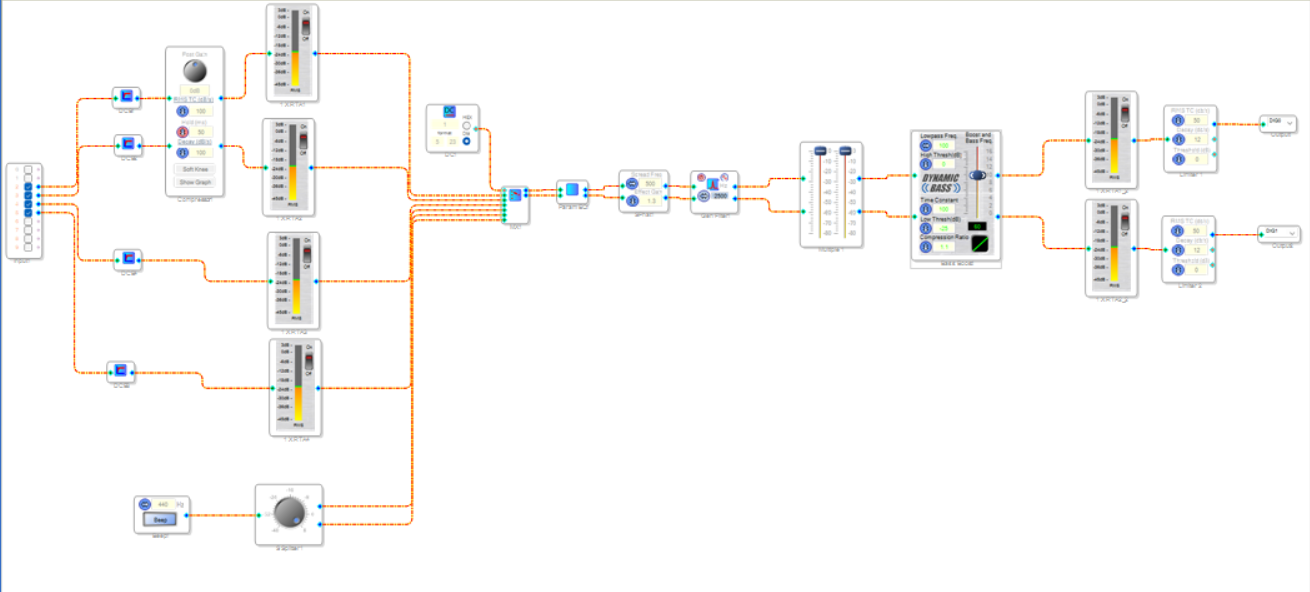
\includegraphics[width=\linewidth]{sigmastudiofinale.png}
  \caption{DigiRadioFinale signal chain: per-channel DC blockers and RMS
    compressor, four input-side level meters, the 6-leg Param EQ, the
    SuperPhat spatializer, an unconfigured general filter, master volume,
    the Dynamic Bass Boost algorithm, two output-side level meters, and the
    L/R limiters.}
  \label{fig:ss-digiradiofinale}
\end{figure}

\begin{table}[htbp]
  \centering
  \small
  \begin{tabular}{@{}L{2.6cm}L{2.2cm}L{7.6cm}@{}}
    \drhead Addresses & Block & Role \\
    \midrule
    0--2    & Beep1        & test tone (unchanged) \\
    3       & DC1          & input trim \\
    4--7    & DCB1--4      & DC blocker, one per channel \\
    8       & S Splitter1  & control fan-out (unchanged) \\
    9--46   & Compressor1  & RMS compander, 34-point curve \\
    47--58  & 1×RTA3,4,1,2 & 4 input-side level meters (readback) \\
    59--88  & Param EQ1    & 6 stereo legs (ST0--ST5) $\times$ 5 coefficients \\
    89--140 & SPhat1       & SuperPhat spatializer (dedicated algorithm,
                              replaces the stereo-enhance EQ overlay) \\
    141--145& Gen Filter1  & general 2nd-order filter, currently flat/bypassed
                              --- reserved, not yet configured (candidate slot
                              for Voice Clarifier) \\
    146--147& Multiple1    & master volume L/R (unchanged) \\
    148--187& Bass Boost1  & Dynamic Bass Boost algorithm (dedicated,
                              replaces the bass-enhance EQ overlay) \\
    188--193& 1×RTA2\_2,1\_2 & 2 output-side level meters (readback) \\
    194--223& Limiter2, Limiter1 & unchanged \\
    \bottomrule
  \end{tabular}
  \caption{DigiRadioFinale parameter RAM map, by address.}
  \label{tab:ss-digiradiofinale-map}
\end{table}

No dedicated mute cell exists yet in this export, and Gen Filter1 (the
Voice Clarifier candidate) is still an identity filter (b0=1, all other
coefficients zero). Both are pending further SigmaStudio work before this
program replaces the one described earlier in this chapter.
